
%(BEGIN_QUESTION)
% Copyright 2007, Tony R. Kuphaldt, released under the Creative Commons Attribution License (v 1.0)
% This means you may do almost anything with this work of mine, so long as you give me proper credit

Assuming a constant setpoint, determine the proportional band setting of the proportional-only controller, as well as its control action (either {\it direct} or {\it reverse}) based on this chart recording of its behavior:

$$\includegraphics[width=15.5cm]{i01499x01.eps}$$

\underbar{file i01499}
%(END_QUESTION)





%(BEGIN_ANSWER)

Proportional band = 66.67\% ; reverse-acting control

%(END_ANSWER)





%(BEGIN_NOTES)

We can see that this controller is reverse-acting because the output decreases in response to an increasing PV, and vice-versa.

\vskip 10pt

Gain is defined as the ratio of output change to input change, so:

$$K_p = {\Delta m \over \Delta \hbox{PV}} = {70 - 62.5 \over 55 - 50} = 1.5$$

$$\hbox{Proportional Band} = {1 \over K_p} = {1 \over 1.5} = 66.67\%$$

%INDEX% Control, proportional: graphing controller response

%(END_NOTES)


